\chapter{Evaluation}

\section{Document management}

In this section, we take \autoref{tab:background-comparison} as a starting
point and check what features are implemented and what are not.

The testing environment was built from a client machine, a SharePoint server
and an Alfresco server, as can be seen on \autoref{fig:test-arch}.

\begin{figure}[H]
\centering
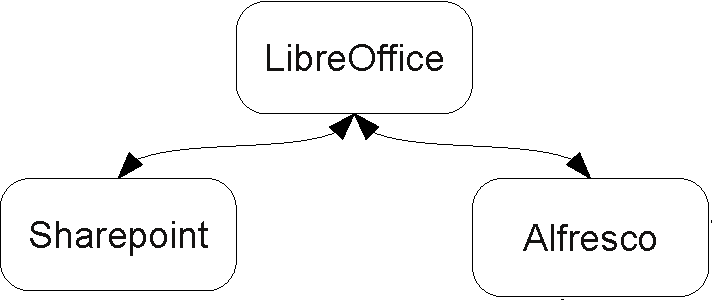
\includegraphics[width=300px,keepaspectratio]{test-arch.pdf}
\caption{Architecture of the test system}
\label{fig:test-arch}
\end{figure}

The client machine had the following details:
\begin{itemize}
\item Frugalware Linux 1.5 (English and Hungarian locale)
\item LibreOffice 3.4, LibreOffice 3.3, OpenOffice.org 3.3 and OpenOffice.org 3.2.1
\end{itemize}

Properties of the SharePoint machine:

\begin{itemize}
\item Microsoft Windows Windows Server 2003 R2 Enterprise (English)
\item Microsoft SharePoint 2007 Enterprise
\end{itemize}

Finally the Alfresco machine:

\begin{itemize}
\item Fedora Linux 16
\item Alfresco 3.4.d Community Edition
\end{itemize}

Regarding functionality, all items from the feature table are implemented in
the extension. The following areas are missing from the table, and not
supported at the moment:

\begin{itemize}
\item User management, including roles and permissions inside workspaces.
\item Task management in workspaces.
\item Link management in workspaces.
\end{itemize}

The following items are not in the feature table, but are available:

\begin{itemize}
\item Creating and deleting workspaces is supported by Microsoft Office, but nested
folder structures can only be read. It turned out that the protocol allows
creation, so the extension supports this.
\item Namespaces of settings and classes are renamed, so parallel installation
of our extension and OPAL is possible.
\end{itemize}

The extension is written in Java and BASIC, so it is meant to be portable.
LibreOffice is available on Windows and OSX as well -- so the extension should
work there, but we only had time to test it on Windows.

Regarding localization, all user-visible strings are externalized to Java
property files. During development we paid attention to English strings, then at
the end as a demonstration we created the Hungarian translation as well. Adding
new translations is easy.

Finally, the extension inherited some of the limitations of the original OPAL
codebase:

\begin{itemize}
\item The GUI is not started in a separate thread in all cases, so in many cases
the user interface is not updated in the background.
\item Classes we did not touch still have French comments inside.
\end{itemize}

\section{Workflows}

\subsection*{Test architecture}

The evaluation of workflow support is based on the use-cases of the workflow
part of the \emph{Overview of the Approach} chapter.

\begin{figure}[H]
\centering
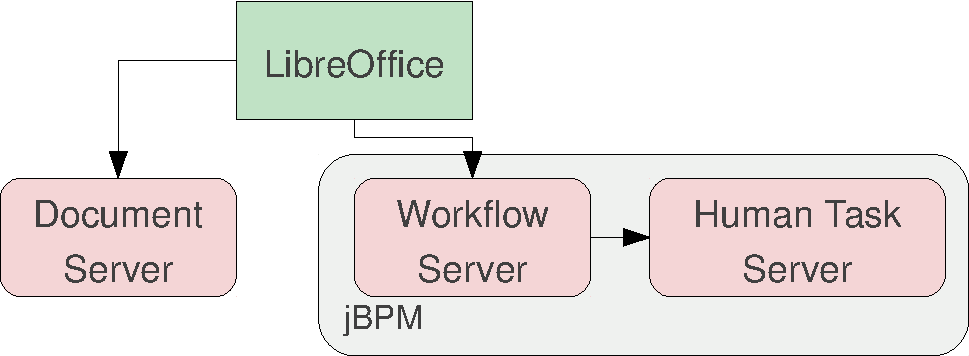
\includegraphics[width=300px,keepaspectratio]{test-arch-wf.pdf}
\caption{Architecture of the workflow-enabled test system}
\label{fig:test-arch-wf}
\end{figure}

We designed a test architecture to evaluate these features, and
\autoref{fig:test-arch-wf} shows the structure of this test environment. The
test system has the following dependencies:

\begin{itemize}
\item The connection should be initiated from our LibreOffice extension when
both the document server and the workflow engine is ready.
\item The workflow server can be started before the Human Task server, but user
connections can only be served when both are ready.
\item Additionally, in case a custom storage backend is used for jBPM (for
example MySQL instead of the default H2 backend), then that should be ready
before any component of jBPM is started.
\end{itemize}

During our tests we used the same document servers and office suites than for
the document-server-only tests. The jBPM instance was set up on the same
physical machine where the office suite ran.

The workflow-specific tests were executed using the following component versions:

\begin{itemize}
\item jBPM (jbpm-bpmn2 and jbpm-human-task) 5.1.x: latest version at the time
of writing (November 2011) with additional patches detailed earlier.
\item BPM Console 2.1 with the patches.
\item MySQL 5.5.14 without additional modifications.
\end{itemize}

The jBPM developers are looking forward to the modifications and are planning
to review them once the thesis is ready.

\subsection*{Used test methods}

Three different test methods were used:

\begin{itemize}
\item The existing document management unit tests were used to ensure that we do not break the document-management-only use cases (see \autoref{tab:background-comparison}).
\item Separate command-line applications were used to test features of the workflow library. These are to be turned into unit tests.
\item Due to the complex architecture, integration tests were performed manually.
\end{itemize}

The last method does not only mean it was continuously tested by the author: a closed set of users also tested it once the document management part was ready. They were already used to using a document server and office suite separately, and they all had the possibility not to use the extension if they thought it complicated their daily work. The general feedback was:

\begin{itemize}
\item The extension made their work easier: in most cases they did use the extension once it was installed.
\item Even if they had to report bugs here and there, the extension never
damaged data on the servers (e.g. by accidentally deleting a version of a
document).
\end{itemize}

\subsection*{Limitations}

The workflow support part has the following known limitations:

\begin{itemize}
\item Process definitions without a start form -- where the associated document URL can be specified -- are not supported.
\item Free-form HTML is not allowed in task forms when making a business decision.
\item The audit log features are not available with an official jBPM version.
\end{itemize}

The first two are design decisions, the last one will be resolved in the near
future, as mentioned earlier.

However the document management integration also causes two limitations, which affects workflows as well:

\begin{itemize}
\item The SharePoint protocol does not allow listing files without an
extension. This means when using the extension to start a workflow, such files
can't be associated to the process instance.
\item By choosing a decoupled approach, we also require an external method to
be used for keeping user accounts on the document management and workflow
servers in sync.
\end{itemize}

Here the first item is a known limitation, the second one is a design decision.
